\pdfbookmark{Общая характеристика работы}{characteristic}             % Закладка pdf
\section*{Общая характеристика работы}

\newcommand{\actuality}{\pdfbookmark[1]{Актуальность}{actuality}\underline{\textbf{\actualityTXT}}}
\newcommand{\progress}{\pdfbookmark[1]{Разработанность темы}{progress}\underline{\textbf{\progressTXT}}}
\newcommand{\aim}{\pdfbookmark[1]{Цели}{aim}\underline{{\textbf\aimTXT}}}
\newcommand{\tasks}{\pdfbookmark[1]{Задачи}{tasks}\underline{\textbf{\tasksTXT}}}
\newcommand{\aimtasks}{\pdfbookmark[1]{Цели и задачи}{aimtasks}\aimtasksTXT}
\newcommand{\novelty}{\pdfbookmark[1]{Научная новизна}{novelty}\underline{\textbf{\noveltyTXT}}}
\newcommand{\influence}{\pdfbookmark[1]{Практическая значимость}{influence}\underline{\textbf{\influenceTXT}}}
\newcommand{\methods}{\pdfbookmark[1]{Методология и методы исследования}{methods}\underline{\textbf{\methodsTXT}}}
\newcommand{\defpositions}{\pdfbookmark[1]{Положения, выносимые на защиту}{defpositions}\underline{\textbf{\defpositionsTXT}}}
\newcommand{\reliability}{\pdfbookmark[1]{Достоверность}{reliability}\underline{\textbf{\reliabilityTXT}}}
\newcommand{\probation}{\pdfbookmark[1]{Апробация}{probation}\underline{\textbf{\probationTXT}}}
\newcommand{\contribution}{\pdfbookmark[1]{Личный вклад}{contribution}\underline{\textbf{\contributionTXT}}}
\newcommand{\publications}{\pdfbookmark[1]{Публикации}{publications}\underline{\textbf{\publicationsTXT}}}


{\actuality} Обзор, введение в тему, обозначение места данной работы в
мировых исследованиях и~т.\:п., можно использовать ссылки на~другие
работы~\autocite{Gosele1999161,Lermontov}
(если их~нет, то~в~автореферате
автоматически пропадёт раздел <<Список литературы>>). Внимание! Ссылки
на~другие работы в~разделе общей характеристики работы можно
использовать только при использовании \verb!biblatex! (из-за технических
ограничений \verb!bibtex8!. Это связано с тем, что одна
и~та~же~характеристика используются и~в~тексте диссертации, и в
автореферате. В~последнем, согласно ГОСТ, должен присутствовать список
работ автора по~теме диссертации, а~\verb!bibtex8! не~умеет выводить в~одном
файле два списка литературы).
При использовании \verb!biblatex! возможно использование исключительно
в~автореферате подстрочных ссылок
для других работ командой \verb!\autocite!, а~также цитирование
собственных работ командой \verb!\cite!. Для этого в~файле
\verb!common/setup.tex! необходимо присвоить положительное значение
счётчику \verb!\setcounter{usefootcite}{1}!.

Для генерации содержимого титульного листа автореферата, диссертации
и~презентации используются данные из файла \verb!common/data.tex!. Если,
например, вы меняете название диссертации, то оно автоматически
появится в~итоговых файлах после очередного запуска \LaTeX. Согласно
ГОСТ 7.0.11-2011 <<5.1.1 Титульный лист является первой страницей
диссертации, служит источником информации, необходимой для обработки и
поиска документа>>. Наличие логотипа организации на~титульном листе
упрощает обработку и~поиск, для этого разметите логотип вашей
организации в папке images в~формате PDF (лучше найти его в векторном
варианте, чтобы он хорошо смотрелся при печати) под именем
\verb!logo.pdf!. Настроить размер изображения с логотипом можно
в~соответствующих местах файлов \verb!title.tex!  отдельно для
диссертации и автореферата. Если вам логотип не~нужен, то просто
удалите файл с~логотипом.

\ifsynopsis
Этот абзац появляется только в~автореферате.
Для формирования блоков, которые будут обрабатываться только в~автореферате,
заведена проверка условия \verb!\!\verb!ifsynopsis!.
Значение условия задаётся в~основном файле документа (\verb!synopsis.tex! для
автореферата).
\else
Этот абзац появляется только в~диссертации.
Через проверку условия \verb!\!\verb!ifsynopsis!, задаваемого в~основном файле
документа (\verb!dissertation.tex! для диссертации), можно сделать новую
команду, обеспечивающую появление цитаты в~диссертации, но~не~в~автореферате.
\fi

% {\progress}
% Этот раздел должен быть отдельным структурным элементом по
% ГОСТ, но он, как правило, включается в описание актуальности
% темы. Нужен он отдельным структурынм элемементом или нет ---
% смотрите другие диссертации вашего совета, скорее всего не нужен.

{\aim} данной работы является \ldots

Для~достижения поставленной цели необходимо было решить следующие {\tasks}:
\begin{enumerate}[beginpenalty=10000] % https://tex.stackexchange.com/a/476052/104425
  \item Исследовать, разработать, вычислить и~т.\:д. и~т.\:п.
  \item Исследовать, разработать, вычислить и~т.\:д. и~т.\:п.
  \item Исследовать, разработать, вычислить и~т.\:д. и~т.\:п.
  \item Исследовать, разработать, вычислить и~т.\:д. и~т.\:п.
\end{enumerate}


{\novelty}
\begin{enumerate}[beginpenalty=10000] % https://tex.stackexchange.com/a/476052/104425
  \item Впервые \ldots
  \item Впервые \ldots
  \item Было выполнено оригинальное исследование \ldots
\end{enumerate}

{\influence} \ldots

{\methods} \ldots

{\defpositions}
\begin{enumerate}[beginpenalty=10000] % https://tex.stackexchange.com/a/476052/104425
  \item Первое положение
  \item Второе положение
  \item Третье положение
  \item Четвертое положение
\end{enumerate}
В папке Documents можно ознакомиться в решением совета из Томского ГУ
в~файле \verb+Def_positions.pdf+, где обоснованно даются рекомендации
по~формулировкам защищаемых положений.

{\reliability} полученных результатов обеспечивается \ldots \ Результаты находятся в соответствии с результатами, полученными другими авторами.


{\probation}
Основные результаты работы докладывались~на:
перечисление основных конференций, симпозиумов и~т.\:п.

{\contribution} Автор принимал активное участие \ldots

\ifnumequal{\value{bibliosel}}{0}
{%%% Встроенная реализация с загрузкой файла через движок bibtex8. (При желании, внутри можно использовать обычные ссылки, наподобие `\cite{vakbib1,vakbib2}`).
    {\publications} Основные результаты по теме диссертации изложены
    в~XX~печатных изданиях,
    X из которых изданы в журналах, рекомендованных ВАК,
    X "--- в тезисах докладов.
}%
{%%% Реализация пакетом biblatex через движок biber
    \begin{refsection}[bl-author, bl-registered]
        % Это refsection=1.
        % Процитированные здесь работы:
        %  * подсчитываются, для автоматического составления фразы "Основные результаты ..."
        %  * попадают в авторскую библиографию, при usefootcite==0 и стиле `\insertbiblioauthor` или `\insertbiblioauthorgrouped`
        %  * нумеруются там в зависимости от порядка команд `\printbibliography` в этом разделе.
        %  * при использовании `\insertbiblioauthorgrouped`, порядок команд `\printbibliography` в нём должен быть тем же (см. biblio/biblatex.tex)
        %
        % Невидимый библиографический список для подсчёта количества публикаций:
        \ifxetexorluatex\selectlanguage{english}\fi
        \printbibliography[heading=nobibheading, section=1, env=countauthorvak,          keyword=biblioauthorvak]%
        \printbibliography[heading=nobibheading, section=1, env=countauthorwos,          keyword=biblioauthorwos]%
        \printbibliography[heading=nobibheading, section=1, env=countauthorscopus,       keyword=biblioauthorscopus]%
        \printbibliography[heading=nobibheading, section=1, env=countauthorconf,         keyword=biblioauthorconf]%
        \printbibliography[heading=nobibheading, section=1, env=countauthorother,        keyword=biblioauthorother]%
        \printbibliography[heading=nobibheading, section=1, env=countregistered,         keyword=biblioregistered]%
        \printbibliography[heading=nobibheading, section=1, env=countauthorpatent,       keyword=biblioauthorpatent]%
        \printbibliography[heading=nobibheading, section=1, env=countauthorprogram,      keyword=biblioauthorprogram]%
        \printbibliography[heading=nobibheading, section=1, env=countauthor,             keyword=biblioauthor]%
        \printbibliography[heading=nobibheading, section=1, env=countauthorvakscopuswos, filter=vakscopuswos]%
        \printbibliography[heading=nobibheading, section=1, env=countauthorscopuswos,    filter=scopuswos]%
        %
        \nocite{*}\ifxetexorluatex\selectlanguage{russian}\fi%
        %
        {\publications} Основные результаты по теме диссертации изложены в~\arabic{citeauthor}~печатных изданиях,
        \arabic{citeauthorvak} из которых изданы в журналах, рекомендованных ВАК\sloppy%
        \ifnum \value{citeauthorscopuswos}>0%
            , \arabic{citeauthorscopuswos} "--- в~периодических научных журналах, индексируемых Web of~Science и Scopus\sloppy%
        \fi%
        \ifnum \value{citeauthorconf}>0%
            , \arabic{citeauthorconf} "--- в~тезисах докладов.
        \else%
            .
        \fi%
        \ifnum \value{citeregistered}=1%
            \ifnum \value{citeauthorpatent}=1%
                Зарегистрирован \arabic{citeauthorpatent} патент.
            \fi%
            \ifnum \value{citeauthorprogram}=1%
                Зарегистрирована \arabic{citeauthorprogram} программа для ЭВМ.
            \fi%
        \fi%
        \ifnum \value{citeregistered}>1%
            Зарегистрированы\ %
            \ifnum \value{citeauthorpatent}>0%
            \formbytotal{citeauthorpatent}{патент}{}{а}{}\sloppy%
            \ifnum \value{citeauthorprogram}=0 . \else \ и~\fi%
            \fi%
            \ifnum \value{citeauthorprogram}>0%
            \formbytotal{citeauthorprogram}{программ}{а}{ы}{} для ЭВМ.
            \fi%
        \fi%
        % К публикациям, в которых излагаются основные научные результаты диссертации на соискание учёной
        % степени, в рецензируемых изданиях приравниваются патенты на изобретения, патенты (свидетельства) на
        % полезную модель, патенты на промышленный образец, патенты на селекционные достижения, свидетельства
        % на программу для электронных вычислительных машин, базу данных, топологию интегральных микросхем,
        % зарегистрированные в установленном порядке.(в ред. Постановления Правительства РФ от 21.04.2016 N 335)
    \end{refsection}%
    \begin{refsection}[bl-author, bl-registered]
        % Это refsection=2.
        % Процитированные здесь работы:
        %  * попадают в авторскую библиографию, при usefootcite==0 и стиле `\insertbiblioauthorimportant`.
        %  * ни на что не влияют в противном случае
        \nocite{vakbib2}%vak
        \nocite{patbib1}%patent
        \nocite{progbib1}%program
        \nocite{bib1}%other
        \nocite{confbib1}%conf
    \end{refsection}%
        %
        % Всё, что вне этих двух refsection, это refsection=0,
        %  * для диссертации - это нормальные ссылки, попадающие в обычную библиографию
        %  * для автореферата:
        %     * при usefootcite==0, ссылка корректно сработает только для источника из `external.bib`. Для своих работ --- напечатает "[0]" (и даже Warning не вылезет).
        %     * при usefootcite==1, ссылка сработает нормально. В авторской библиографии будут только процитированные в refsection=0 работы.
}

При использовании пакета \verb!biblatex! будут подсчитаны все работы, добавленные
в файл \verb!biblio/author.bib!. Для правильного подсчёта работ в~различных
системах цитирования требуется использовать поля:
\begin{itemize}
        \item \texttt{authorvak} если публикация индексирована ВАК,
        \item \texttt{authorscopus} если публикация индексирована Scopus,
        \item \texttt{authorwos} если публикация индексирована Web of Science,
        \item \texttt{authorconf} для докладов конференций,
        \item \texttt{authorpatent} для патентов,
        \item \texttt{authorprogram} для зарегистрированных программ для ЭВМ,
        \item \texttt{authorother} для других публикаций.
\end{itemize}
Для подсчёта используются счётчики:
\begin{itemize}
        \item \texttt{citeauthorvak} для работ, индексируемых ВАК,
        \item \texttt{citeauthorscopus} для работ, индексируемых Scopus,
        \item \texttt{citeauthorwos} для работ, индексируемых Web of Science,
        \item \texttt{citeauthorvakscopuswos} для работ, индексируемых одной из трёх баз,
        \item \texttt{citeauthorscopuswos} для работ, индексируемых Scopus или Web of~Science,
        \item \texttt{citeauthorconf} для докладов на конференциях,
        \item \texttt{citeauthorother} для остальных работ,
        \item \texttt{citeauthorpatent} для патентов,
        \item \texttt{citeauthorprogram} для зарегистрированных программ для ЭВМ,
        \item \texttt{citeauthor} для суммарного количества работ.
\end{itemize}
% Счётчик \texttt{citeexternal} используется для подсчёта процитированных публикаций;
% \texttt{citeregistered} "--- для подсчёта суммарного количества патентов и программ для ЭВМ.

Для добавления в список публикаций автора работ, которые не были процитированы в
автореферате, требуется их~перечислить с использованием команды \verb!\nocite! в
\verb!Synopsis/content.tex!.
 % Характеристика работы по структуре во введении и в автореферате не отличается (ГОСТ Р 7.0.11, пункты 5.3.1 и 9.2.1), потому её загружаем из одного и того же внешнего файла, предварительно задав форму выделения некоторым параметрам

%Диссертационная работа была выполнена при поддержке грантов \dots

%\underline{\textbf{Объем и структура работы.}} Диссертация состоит из~введения,
%четырех глав, заключения и~приложения. Полный объем диссертации
%\textbf{ХХХ}~страниц текста с~\textbf{ХХ}~рисунками и~5~таблицами. Список
%литературы содержит \textbf{ХХX}~наименование.

\pdfbookmark{Содержание работы}{description}                          % Закладка pdf
\section*{Содержание работы}
Во \underline{\textbf{введении}} обосновывается актуальность
исследований, проводимых в~рамках данной диссертационной работы,
приводится обзор научной литературы по~изучаемой проблеме,
формулируется цель, ставятся задачи работы, излагается научная новизна
и практическая значимость представляемой работы. В~последующих главах
сначала описывается общий принцип, позволяющий \dots, а~потом идёт
апробация на частных примерах: \dots  и~\dots.


\underline{\textbf{Первая глава}} посвящена \dots

картинку можно добавить так:
\begin{figure}[ht]
    \centerfloat{
        \hfill
        \subcaptionbox{\LaTeX}{%
            
\includegraphics[scale=0.27]{latex}}
        \hfill
        \subcaptionbox{Knuth}{%
            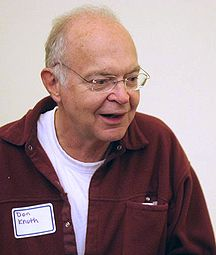
\includegraphics[width=0.25\linewidth]{knuth1}}
        \hfill
    }
    \caption{Подпись к картинке.}\label{fig:latex}
\end{figure}

Формулы в строку без номера добавляются так:
\[
  \lambda_{T_s} = K_x\frac{d{x}}{d{T_s}}, \qquad
  \lambda_{q_s} = K_x\frac{d{x}}{d{q_s}},
\]

\underline{\textbf{Вторая глава}} посвящена исследованию

\underline{\textbf{Третья глава}} посвящена исследованию

Можно сослаться на свои работы в автореферате. Для этого в файле
\verb!Synopsis/setup.tex! необходимо присвоить положительное значение
счётчику \verb!\setcounter{usefootcite}{1}!. В таком случае ссылки на
работы других авторов будут подстрочными.
Изложенные в третьей главе результаты опубликованы в~\cite{vakbib1, vakbib2}.
Использование подстрочных ссылок внутри таблиц может вызывать проблемы.

В \underline{\textbf{четвертой главе}} приведено описание

\FloatBarrier
\pdfbookmark{Заключение}{conclusion}                                  % Закладка pdf
В \underline{\textbf{заключении}} приведены основные результаты работы, которые заключаются в следующем:
%% Согласно ГОСТ Р 7.0.11-2011:
%% 5.3.3 В заключении диссертации излагают итоги выполненного исследования, рекомендации, перспективы дальнейшей разработки темы.
%% 9.2.3 В заключении автореферата диссертации излагают итоги данного исследования, рекомендации и перспективы дальнейшей разработки темы.
\begin{enumerate}
  \item На основе анализа \ldots
  \item Численные исследования показали, что \ldots
  \item Математическое моделирование показало \ldots
  \item Для выполнения поставленных задач был создан \ldots
\end{enumerate}


\pdfbookmark{Литература}{bibliography}                                % Закладка pdf
При использовании пакета \verb!biblatex! список публикаций автора по теме
диссертации формируется в разделе <<\publications>>\ файла
\verb!common/characteristic.tex!  при помощи команды \verb!\nocite!

\ifdefmacro{\microtypesetup}{\microtypesetup{protrusion=false}}{} % не рекомендуется применять пакет микротипографики к автоматически генерируемому списку литературы
\urlstyle{rm}                               % ссылки URL обычным шрифтом
\ifnumequal{\value{bibliosel}}{0}{% Встроенная реализация с загрузкой файла через движок bibtex8
  \renewcommand{\bibname}{\large \bibtitleauthor}
  \nocite{*}
  \insertbiblioauthor           % Подключаем Bib-базы
  %\insertbiblioexternal   % !!! bibtex не умеет работать с несколькими библиографиями !!!
}{% Реализация пакетом biblatex через движок biber
  % Цитирования.
  %  * Порядок перечисления определяет порядок в библиографии (только внутри подраздела, если `\insertbiblioauthorgrouped`).
  %  * Если не соблюдать порядок "как для \printbibliography", нумерация в `\insertbiblioauthor` будет кривой.
  %  * Если цитировать каждый источник отдельной командой --- найти некоторые ошибки будет проще.
  %
  %% authorvak
  \nocite{vakbib1}%
  \nocite{vakbib2}%
  %
  %% authorwos
  \nocite{wosbib1}%
  %
  %% authorscopus
  \nocite{scbib1}%
  %
  %% authorpathent
  \nocite{patbib1}%
  %
  %% authorprogram
  \nocite{progbib1}%
  %
  %% authorconf
  \nocite{confbib1}%
  \nocite{confbib2}%
  %
  %% authorother
  \nocite{bib1}%
  \nocite{bib2}%

  \ifnumgreater{\value{usefootcite}}{0}{
    \begin{refcontext}[labelprefix={}]
      \ifnum \value{bibgrouped}>0
        \insertbiblioauthorgrouped    % Вывод всех работ автора, сгруппированных по источникам
      \else
        \insertbiblioauthor      % Вывод всех работ автора
      \fi
    \end{refcontext}
  }{
  \ifnum \totvalue{citeexternal}>0
    \begin{refcontext}[labelprefix=A]
      \ifnum \value{bibgrouped}>0
        \insertbiblioauthorgrouped    % Вывод всех работ автора, сгруппированных по источникам
      \else
        \insertbiblioauthor      % Вывод всех работ автора
      \fi
    \end{refcontext}
  \else
    \ifnum \value{bibgrouped}>0
      \insertbiblioauthorgrouped    % Вывод всех работ автора, сгруппированных по источникам
    \else
      \insertbiblioauthor      % Вывод всех работ автора
    \fi
  \fi
  %  \insertbiblioauthorimportant  % Вывод наиболее значимых работ автора (определяется в файле characteristic во второй section)
  \begin{refcontext}[labelprefix={}]
      \insertbiblioexternal            % Вывод списка литературы, на которую ссылались в тексте автореферата
  \end{refcontext}
  % Невидимый библиографический список для подсчёта количества внешних публикаций
  % Используется, чтобы убрать приставку "А" у работ автора, если в автореферате нет
  % цитирований внешних источников.
  \printbibliography[heading=nobibheading, section=0, env=countexternal, keyword=biblioexternal, resetnumbers=true]%
  }
}
\ifdefmacro{\microtypesetup}{\microtypesetup{protrusion=true}}{}
\urlstyle{tt}                               % возвращаем установки шрифта ссылок URL
